\section{Phase-1 visual summary}
\label{sec:phase1_visual_summary}
The preceding sections report Phase~1 primarily through equations, convergence statistics, and sensitivity tables. This section collects a compact visual summary of the same version-controlled evidence. The figures are not additional experiments; they visualize the existing P1A, P1C, P1D, P1F-C, and P1F-D results in a form that makes estimator behavior, geometry effects, and matched method differences easier to inspect.

\subsection{Known-pose IMU--UWB baseline}
Figure~\ref{fig:p1a_visual} shows the representative P1A trajectory together with its position-error history. The noisy inertial dead-reckoning trajectory gradually departs from the reference, whereas the PF using the synchronous UWB ranges remains much closer over the complete trajectory. This visualization supports the numerical P1A/P1B conclusion that the present UWB fusion primarily acts as a position-drift correction mechanism in the approximately known-pose setting.

\begin{figure}[htbp]
    \centering
    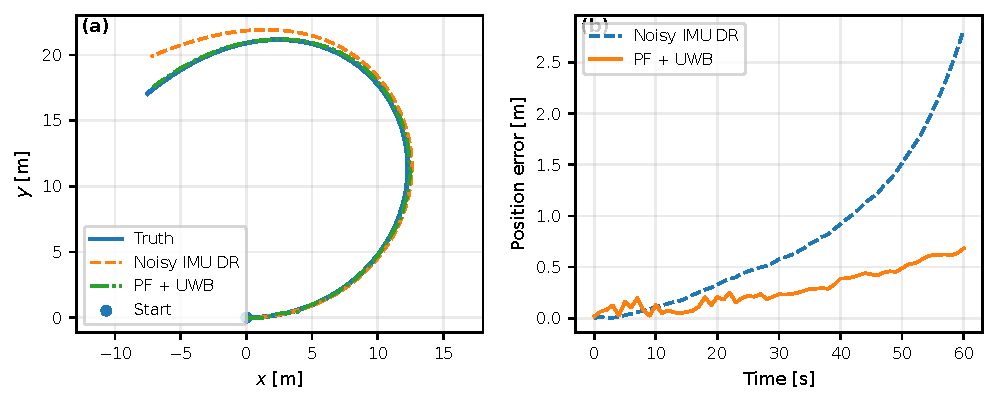
\includegraphics[width=0.98\textwidth]{figures/phase1/p1a_baseline_trajectory.pdf}
    \caption{P1A representative known-pose baseline. (a) Ground-truth trajectory, noisy IMU dead reckoning, and PF+UWB estimate for the committed seed-42 result. (b) Corresponding position-error histories. The figure visualizes the same run summarized numerically in Table~\ref{tab:p1results}.}
    \label{fig:p1a_visual}
\end{figure}

\subsection{Unknown-pose bootstrap-PF sensitivity}
Figure~\ref{fig:p1c_visual} summarizes two P1C sensitivity sweeps. Increasing the global particle population changes the late error but does not yield a monotonic increase in terminal pose success. Likewise, changing the conventional resampling threshold alters the selected realization outcomes but does not remove the low global-pose success rate. The visual summary therefore reinforces the P1C conclusion that the main failure is not explained by one insufficient particle count or by one conventional resampling threshold.

\begin{figure}[htbp]
    \centering
    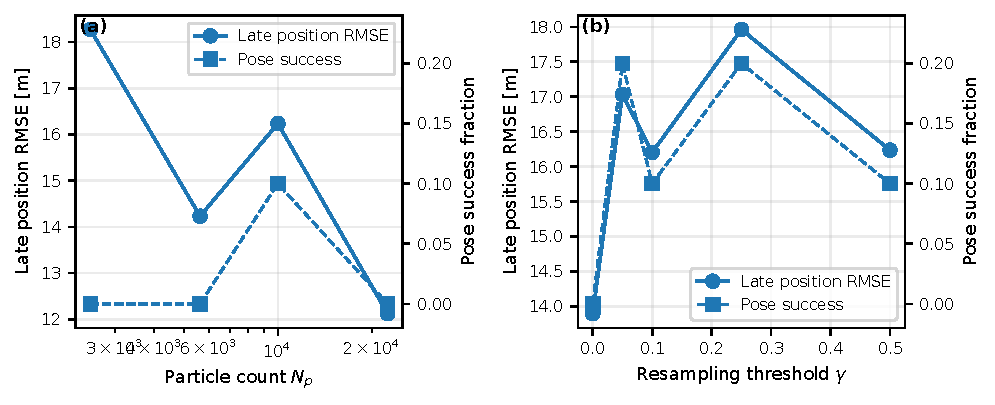
\includegraphics[width=0.98\textwidth]{figures/phase1/p1c_global_search_sensitivity.pdf}
    \caption{P1C unknown-pose bootstrap-PF sensitivity. (a) Late position RMSE and terminal pose-success fraction versus particle population. (b) The same quantities versus the effective-sample-size resampling threshold $\gamma$. Neither sweep provides a monotonic solution to the global-mode-selection problem.}
    \label{fig:p1c_visual}
\end{figure}

\subsection{Geometry, observability, and localization error}
Figure~\ref{fig:p1d_visual} makes the P1D geometry result explicit in the time domain. The stationary and synthetic constant-bearing cases retain an effectively zero normalized smallest singular value over the finite horizon, whereas the informative moving auxiliary eventually reaches the diagnostic conditioning level $\eta_{\mathcal O}=10^{-4}$. The corresponding filtering error histories show that the rank-deficient geometries and the locally full-rank moving case lead to qualitatively different behavior. The moving case remains difficult, but it is the only one in which full-pose recovery is supported by the local finite-horizon information structure.

\begin{figure}[htbp]
    \centering
    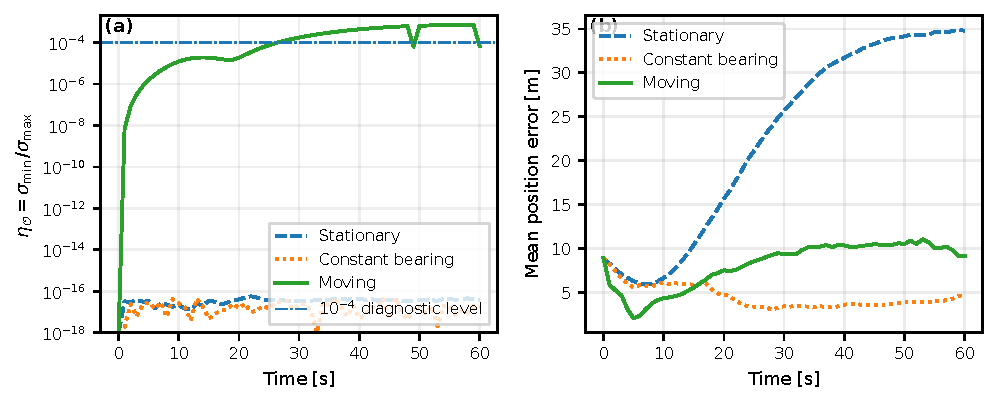
\includegraphics[width=0.98\textwidth]{figures/phase1/p1d_geometry_observability.pdf}
    \caption{P1D geometry and observability diagnostic. (a) Normalized finite-horizon observability conditioning $\eta_{\mathcal O}=\sigma_{\min}/\sigma_{\max}$ for the stationary, constant-bearing, and informative moving auxiliary trajectories. (b) Mean position-error histories of the corresponding realistic global-pose PF campaigns.}
    \label{fig:p1d_visual}
\end{figure}

\subsection{Safety-aware AACOPF tuning}
Figure~\ref{fig:p1fc_visual} visualizes the P1F-C development sweep over $(\alpha,\beta,c_\lambda)$. The selected tuple $(0.5,0,2)$ lies in a region with high correct-mode lock and low wrong-mode-lock/catastrophic-collapse incidence relative to the more aggressive configurations. The figure also illustrates why the tuning criterion cannot be based on localization success alone: several settings attain useful correct-lock fractions while simultaneously producing frequent genealogical collapse.

\begin{figure}[htbp]
    \centering
    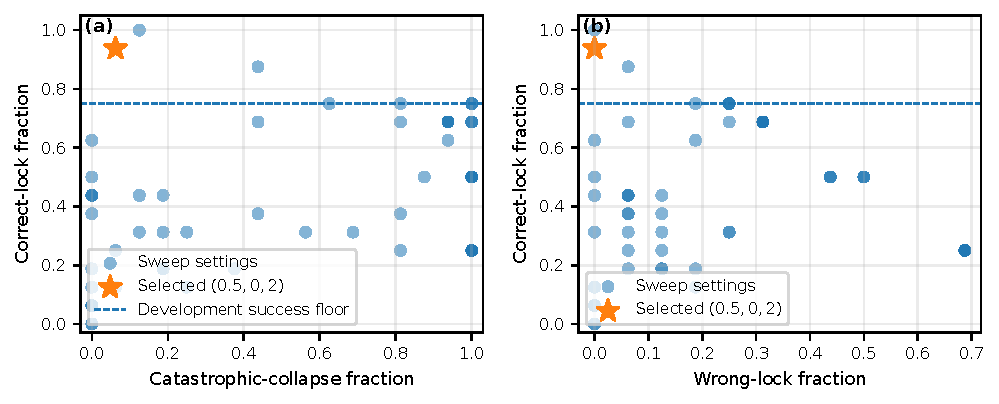
\includegraphics[width=0.98\textwidth]{figures/phase1/p1fc_tuning_tradeoff.pdf}
    \caption{P1F-C development-sweep trade-off. Each point is one of the 60 audited literal-small AACOPF settings. Correct-mode lock is shown against (a) catastrophic ancestry-collapse fraction and (b) wrong-mode-lock fraction. The star denotes the frozen tuple $(\alpha,\beta,c_\lambda)=(0.5,0,2)$; the dashed horizontal line is the predefined $0.75$ development success floor.}
    \label{fig:p1fc_visual}
\end{figure}

\subsection{Matched PF--AACOPF comparison}
Figure~\ref{fig:p1fd_visual} shows the held-out paired P1F-D errors at the primary $N_p=1200$ budget. Points below the diagonal correspond to matched seeds for which AACOPF has lower late error than the conventional PF. AACOPF reduces late position RMSE in $65\%$ of the pairs and late yaw RMSE in $70\%$, consistent with the aggregate error-shaping effect reported in P1F-D. At the same time, strict pose convergence remains $2/20$ for PF and $1/20$ for AACOPF. The visual comparison therefore supports the deliberately limited claim: the frozen literal AACOPF often selects a closer global mode, but it does not improve the strict global-convergence rate under sparse random-annulus support.

\begin{figure}[htbp]
    \centering
    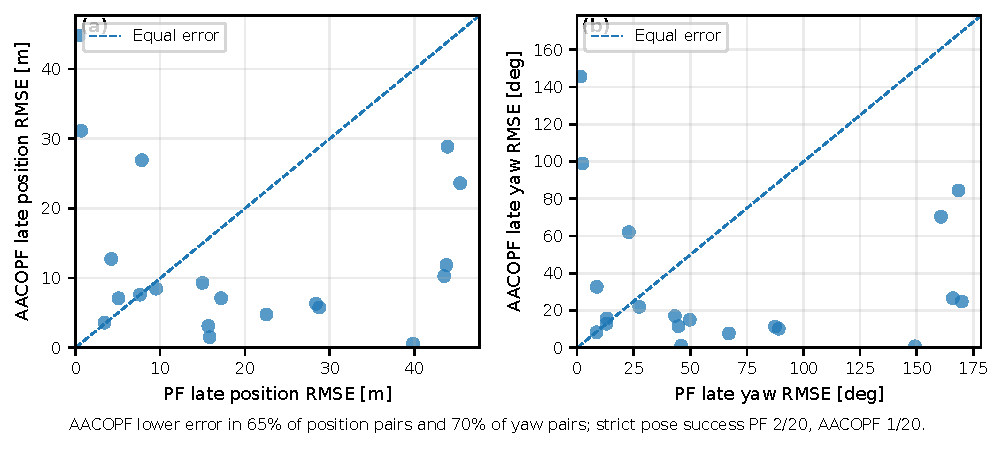
\includegraphics[width=0.98\textwidth]{figures/phase1/p1fd_matched_pf_aacopf.pdf}
    \caption{P1F-D held-out matched comparison at $N_p=1200$. Each point is one common random-annulus initialization and UWB-noise realization. (a) Late position RMSE and (b) late yaw RMSE for conventional PF versus frozen AACOPF. Points below the dashed equality line favor AACOPF.}
    \label{fig:p1fd_visual}
\end{figure}

\subsection{Figure reproducibility}
The compact figure set is generated by \texttt{experiments/generate\_report\_figures.py}. The P1A trajectory report and P1C aggregate summary were already version controlled. For the visual summary, compact report-level data extracts are additionally version controlled for the P1D time histories, the complete P1F-C development sweep, and the P1F-D matched $N_p=1200$ runs. These extracts are derived without changing the underlying experiment outcomes and allow the report figures to be regenerated without depending on expiring GitHub Actions artifacts.
